\documentclass[final,journal,letterpaper]{IEEEtran}

\usepackage{cite}
\usepackage{amsmath}
\usepackage{amsfonts}
\usepackage{amssymb}
\usepackage{graphicx}
\usepackage{url}
\usepackage{balance}
\usepackage{float}
\usepackage{threeparttable}

\usepackage[T1]{fontenc}
\usepackage[latin9]{inputenc}
\usepackage{textcomp}
\usepackage{mathrsfs}
\usepackage{amsthm}

\usepackage{mathptmx}
\usepackage[scaled=.90]{helvet}
\usepackage{courier}

\usepackage{listings}
\usepackage{listings}

\lstset{
   language=C,
   basicstyle=\small,
   keywordstyle=\bfseries,
   identifierstyle=\ttfamily,
   stringstyle=\ttfamily,
   numbers=left,
   numberstyle=\tiny,
   stepnumber=1,
   numbersep=-5pt,
   showstringspaces=false
%   frame=single %trbl%
}

\usepackage[normalem]{ulem}

%------------------------------------------------------------------------------

\newcommand{\etal}{\emph{et al.}}
\newcommand{\eg}{\emph{e.g.}}
\newcommand{\ie}{\emph{i.e.}}
\newcommand{\etc}{\emph{etc.}}
\renewcommand{\baselinestretch}{0.98}\normalsize
%------------------------------------------------------------------------------
\makeatletter
%%%%%%%%%%%%%%%%%%%%%%%%%%%%%% Textclass specific LaTeX commands.
\theoremstyle{plain}
\newtheorem{thm}{\protect\theoremname}
\theoremstyle{definition}
\newtheorem{defn}[thm]{\protect\definitionname}
\theoremstyle{remark}
\newtheorem{rem}[thm]{\protect\remarkname}

\makeatother

%\usepackage{babel}
\providecommand{\definitionname}{Definition}
\providecommand{\remarkname}{Remark}
\providecommand{\theoremname}{Theorem}

\begin{document}

\author{Vincenzo~Catania, Andrea Araldo~and~Davide~Patti% 
\thanks{The authors are with the Dipartimento di Ingegneria
Elettrica, Elettronica ed Informatica, Universit\`a di Catania, Italy
(email: \{vincenzo.catania,aaraldo,davide.patti\}@dieei.unict.it).}}

\title{Parameter space representation of Pareto set}
%ATTENZIONE: in questo testo io mi sono riferito a ``Pareto set''
%come un sottoinsieme dello spazio degli obiettivi (vedi, ad es., descrizione
%dell'algoritmo). E' pi� corretto forse, invece, intendere il Pareto
%set come un sottoinsieme dello spazio delle configurazioni.

\maketitle
\begin{abstract}
In this paper ...
\end{abstract}

%------------------------------------------------------------------------------
%\IEEEkeywords{...}

\begin{IEEEkeywords}
Nanotechnology, DNA, Self-assembly, Routing
\end{IEEEkeywords}
%------------------------------------------------------------------------------
\section{Introduction}

The design of an embedded system requires several objectives (energy
consumption, area occupation, ...) to be fulfilled. The fulfilling
of these objectives depends on several parameters and in the real
cases no analytical results are known to show the relation between
configurations (combination of parameters) and objectives. Therefore
the simulation is the only way to have a picture of how parameters
impact on the objectives. The problem is that the number of parameters
and the number of values that each of them may take lead to an enormous
number of possible configurations, such that simulating all of them
is an unfeasible activity. Therefore there is the need for the ``Design
Space Exploration'', i.e. a methodology to select a subset of all
possible configurations and simulate only this subset.

Many different design space exploration algorithms have been proposed.
A design space exploration algorithm is typically not based on precise
/ analytical / mathematical evidences. The motivations of an exploration
algorithm are rather heuristic, have some form of arbitrariness and,
to a large extend, intuition lies behind them.



The result of every design space exploration is a subset of the configurations
called Pareto Set (\cite{pareto}). Roughly speaking, it is a set of
configurations such that there are no other configurations, among
the simulated ones, that have all the objectives, at the same time,
better fulfilled. If all possible configurations were evaluated, the
ideal Pareto set (the ``true'' Pareto set) could be calculated.
But, as stated above, evaluating all the configurations is not feasable.
Therefore the Pareto set returned by an exploration algorithm is an
approximation of the ``true'' Pareto set.

Many exploration algorithms form the resulting Pareto set in an incremental
way. The algorithm adds and removes configurations in Pareto set while
choosing the configurations to evaluate and simulating them. So Pareto
set ``evolves'' towards the final one. The dynamical view of the
Pareto set shaping can be seen as the ``behavior'' of the algorithm.
This behavior tells us how the Pareto set ``converges'' towards
the final Pareto set. 

The ``quality'' of an exploration algorithm involves two aspects:
\begin{itemize}
\item how much the Pareto set returned by the exploration algorithm is similar
to the ``true'' Pareto set (notice that this cannot be evaluated
because the true Pareto set is unknown - it is only an ``ideal''
quality factor)
\item how fast the Pareto set converges towards the final one. If algorithm
$1$ returns the final Pareto set after simulating $n_{1}$ configurations
and algorithm $2$ returns its final Pareto set after $n_{2}$ simulations,
algorithm $1$ is said to be faster than algorithm $2$, iff $n_{1}<n_{2}$.
\end{itemize}

\section{\label{sec:Related-work}Related work}

There are a number of design space exploration algorithms proposed
in literature.

The ``Dependency analysis'' proposed in \cite{givargis_tvlsi02}, is meant
to take advantage of the dependency among the parameters in a multiobjective
optimization problem. It is required that the designer knows, prior
to the exploration, if a parameter X is dependent from a parameter
Y, i.e. changing the value of Y ``impacts the optimal parameter value''
for X. With this a-priori knowledge, the designer can construct a
``dependency graph'' and recognize clusters, i.e. subsets of strongly
dependency-connected parameters. Each cluster is exhaustively evaluated
and its ``local Pareto set'' is found. Then, all local Pareto sets
are merged. Doing this way, a ``sum'' of local exhaustive evaluations
are performed instead of an exhaustive evaluation of all the possible
configurations. Some problems arise: i) In real scenarios, it may
be very difficult to recognize really independent clusters of parameters,
because there may be interdependencies among a very large number of
parameters. This may lead to the need of an exhaustive search through
almost all the possible configurations. ii) A designer may not have
a precise and complete picture of the dependencies among parameters;
for this reason the need of ``automated approaches for computing
{[}...{]} interdependencies'' is declared in the same paper. iii)
There may be some ``local dependencies'', i.e. dependencies that
emerge only if parameter values are bounded to certain ranges.

These drawbacks are not present in our solution. The algorithm presented
here is also meant to take advantage of dependency but is not directly
based on dependency itself, but rather it ``catches'' dependencies
in terms of ``interesting or uninteresting regions''; as a consequence
no a-priori knowledge of dependencies is required as they are discovered
during exploration. Moreover, recognizing regions offers the capability
to capture local dependencies.

Abraham, Rau and Schreiber proposed in \cite{santosh_hptr00} to decompose
the system to be evaluated into components that interact minimally
with each other. ``Alternative designs for each component are evaluated
in isolation to determine the best designs for individual components.
Combinations of these designs are then put together to build the complete
system design''. Pareto sets for each component are found and, provided
that ``monotonicity'' exists, the complete Pareto set is computed
merging the component Pareto sets. Roughly speaking (see section 4
of the same paper for more details), monotonicity property guarantees
that the best system can be obtained as a composition of the best
components. This approach would perfectly work if all the components
were perfectly isolated, i.e., if there were no dependencies among
different components (in a sense similar (but not necesarily equal)
to the one of Dependency analisys). But real scenarios seldom if ever
expose monotonicity property. This leads to some ``inaccuracies''
(as stated in section 4.6.1 of the same paper).

Other approaches take into account the concept of ``sensitivity''.
The sensitivity of an objective with the respect to a parameter is
a measure of how much the objective varies when varying that parameter.
A ``sensitivity analysis'' was used in \cite{fornaciari_codes01} in an optimization
problem with only one objective (the power-delay product of an electronic
device). This method was extended in \cite{palesi_iwsoc02} to a multiobjective
optimization. In that work the sensitivity of objectives with
the respect to each parameter is measured, and parameters are ordered
on the base on these sensitivity measures. Then, a first Pareto set
is obtained varying the first parameter, having fixed to arbitrary
values all other parameters. The Pareto set is then refined varying,
in a similar way, the other parameters, one by one. Experimental results
(see section 4.2 of the same work) show that this method is not of
good ``quality'' (as broadly defined in the introduction). The reason
can be found in the very limited and rigid exploration of the parameter
space: after computing the first Pareto set, there are no more chances
to consider configurations with values of the first parameter other
than the ones assumed in the first Pareto set calculation. Similar
limitations are imposed after computing the second Pareto set, the
third and so on. It is worth noticing that this approach can not capture
``local sensitivity'' (this drawback will be called ``local sensitivity
limitation''), i.e. the objectives may be more sensitive to some
ranges of a parameter and less sensitive to other ranges of the same
parameter. Moreover it can not capture ``combined sensitivity''
(``combined sensitivity limitation''), i.e. the objectives may be
more sensitive to a range of a parameter $p_{1}$, only when other
parameters are within certain ranges, and less sensitive to the same
range of parameter $p_{1}$ when the other parameters are not within
those ranges. Therefore, in the method we propose, we do not use the
sensitivity directly, but we use the concept of innovation (that can
be considered, at least weakly related to the sensitivity). We do
not measure innovation of a parameter (as done for the sensitivity),
but rather we measure the innovation of a ``region'' of parameter
space, in order to overcome both the ``local sensitivity limitation''
and the ``combined sensitivity limitation'' stated above for the
sensitivity analysis.

Many studies focus on genetic approaches to resolve multiobjective
optimization problems (\cite{} and others). Genetic approaches
have many advantages: they have proved good quality (as broadly defined
in the introduction), they are customizable, they are very general
and require no a-priori knowledge to the designer. Genetic algorithms
run in subsequent iterations. Configurations are represented as chromosomes.
In each iteration a ``population'' of configurations is evaluated.
Some configurations are discarded. Each selected configuration is
combined with the preceding population and then ``mutated'' (i.e.
the resulting configuration is varied a little). Iterating this operations,
populations are expected to become ``better and better''. The strong
point of genetic approaches can be summarized saying that they consist
in a broad exploration (the mutation permits to make the exploration
not rigidly restricted to limited parts of parameter space), although
this exploration is not random but is guided by the performances of
the already evaluated configurations. Therefore, the exploration is
neither too much constrained nor too much random. We claim that the
approach presented in this paper has all the benefits of the genetic
approaches, although the rational is completely different.


\section{Preliminaries}


\subsection{Representation}
\begin{defn}
\emph{Configuration}

Let $p_{1},\dots,p_{n}$ be the parameters and $P_{i}$ the domain
of $p_{i}$, i.e. the set of values $v\in P_{i}$ that parameter $p_{i}$
may assume. A configuration is a vector
\[
\mathbf{p}=\left(v_{1},\dots,v_{n}\right)\in P_{1}\times\dots\times P_{n}
\]

\end{defn}

\begin{defn}
\emph{Objective function}

Let $o_{1},\dots,o_{m}$ be the objectives and $O_{i}$ the set of
values that $o_{i}$ may assume. Let $O_{i}$ have a ``better than''
operator $\vartriangleright$ defined so that, taking $o_{i},q_{i}\in O_{i}$,
we can always say:
\[
o_{i}\vartriangleright q_{i}\mbox{ (}o_{i}\mbox{ is better than }q_{i}\mbox{)}
\]
 or
\[
o_{i}\vartriangleleft q_{i}\mbox{ (}o_{i}\mbox{ is worse than }q_{i}\mbox{)}
\]
 or
\[
o_{i}\bowtie q_{i}\mbox{ (}o_{i}\mbox{ is neither better nor worse than }q_{i}\mbox{)}
\]


$o_{i}$ can be viewed as a function
\[
o_{i}:\mathbf{p}\rightarrow o_{i}\left(\mathbf{p}\right)\in O_{i},\ \forall\mathbf{p}\in P_{1}\times\dots\times P_{n}
\]
 To take into account all of the objectives, the following function
is defined:
\[
\mathbf{o}:\mathbf{p}\rightarrow\left(o_{1}\left(\mathbf{p}\right),\dots,o_{m}\left(\mathbf{p}\right)\right),\ \forall\mathbf{p}\in P_{1}\times\dots\times P_{n}
\]

\end{defn}


{[}BISOGNEREBBE INTRODURRE IL CONCETTO DI FEASIBILITY{]}
\begin{defn}
\emph{\label{pers02.def:Pareto-set}Pareto set}

Let $U\subseteq P_{1}\times\dots\times P_{n}$. The set of its dominated
configurations is:
\[
Dom\left(U\right)=\left\{ \left.\mathbf{p}\in U\right|\exists\mathbf{x}\in U:o_{i}\left(\mathbf{x}\right)\vartriangleright o_{i}\left(\mathbf{p}\right),\mbox{for }i=1,\dots m\right\} 
\]


Its Pareto set is defined as:
\[
\mathscr{P}\left(U\right)=U\setminus Dom\left(U\right)
\]


When there is no ambiguity, $\mathscr{P}$ is written instead of $\mathscr{P}\left(U\right)$.
\end{defn}

\begin{defn}
\emph{Pareto front}

The Pareto front is the representation in the objective space of the
Pareto set, i.e.:
\[
\mathbf{o}\left(\mathscr{P}\right)\in O_{1}\times\dots\times O_{m}
\]

\end{defn}
On the contrary, we call ``parameter space representation'' of the
Pareto set the representation in which each configuration $\mathbf{p}$
is simply represented as a point of $P_{1}\times\dots\times P_{n}$
space. We will investigate the relation between the ``objective space
representation'' and the ``parameter space representation''. We
are particularly interested in the relation between the evolution
of the objective space representation of the Pareto set and the evolution
of its parameter space representation.

!!! FORSE NON E' VERO CHE NOI WILL INVESTIGATE .... FORSE IL PERIODO
PRECEDENTE NON VA PIU' BENE PERCHE' NON TROVA RISCONTRO NEL RESTO
DELLA TRATTAZIONE

\begin{figure}[h]
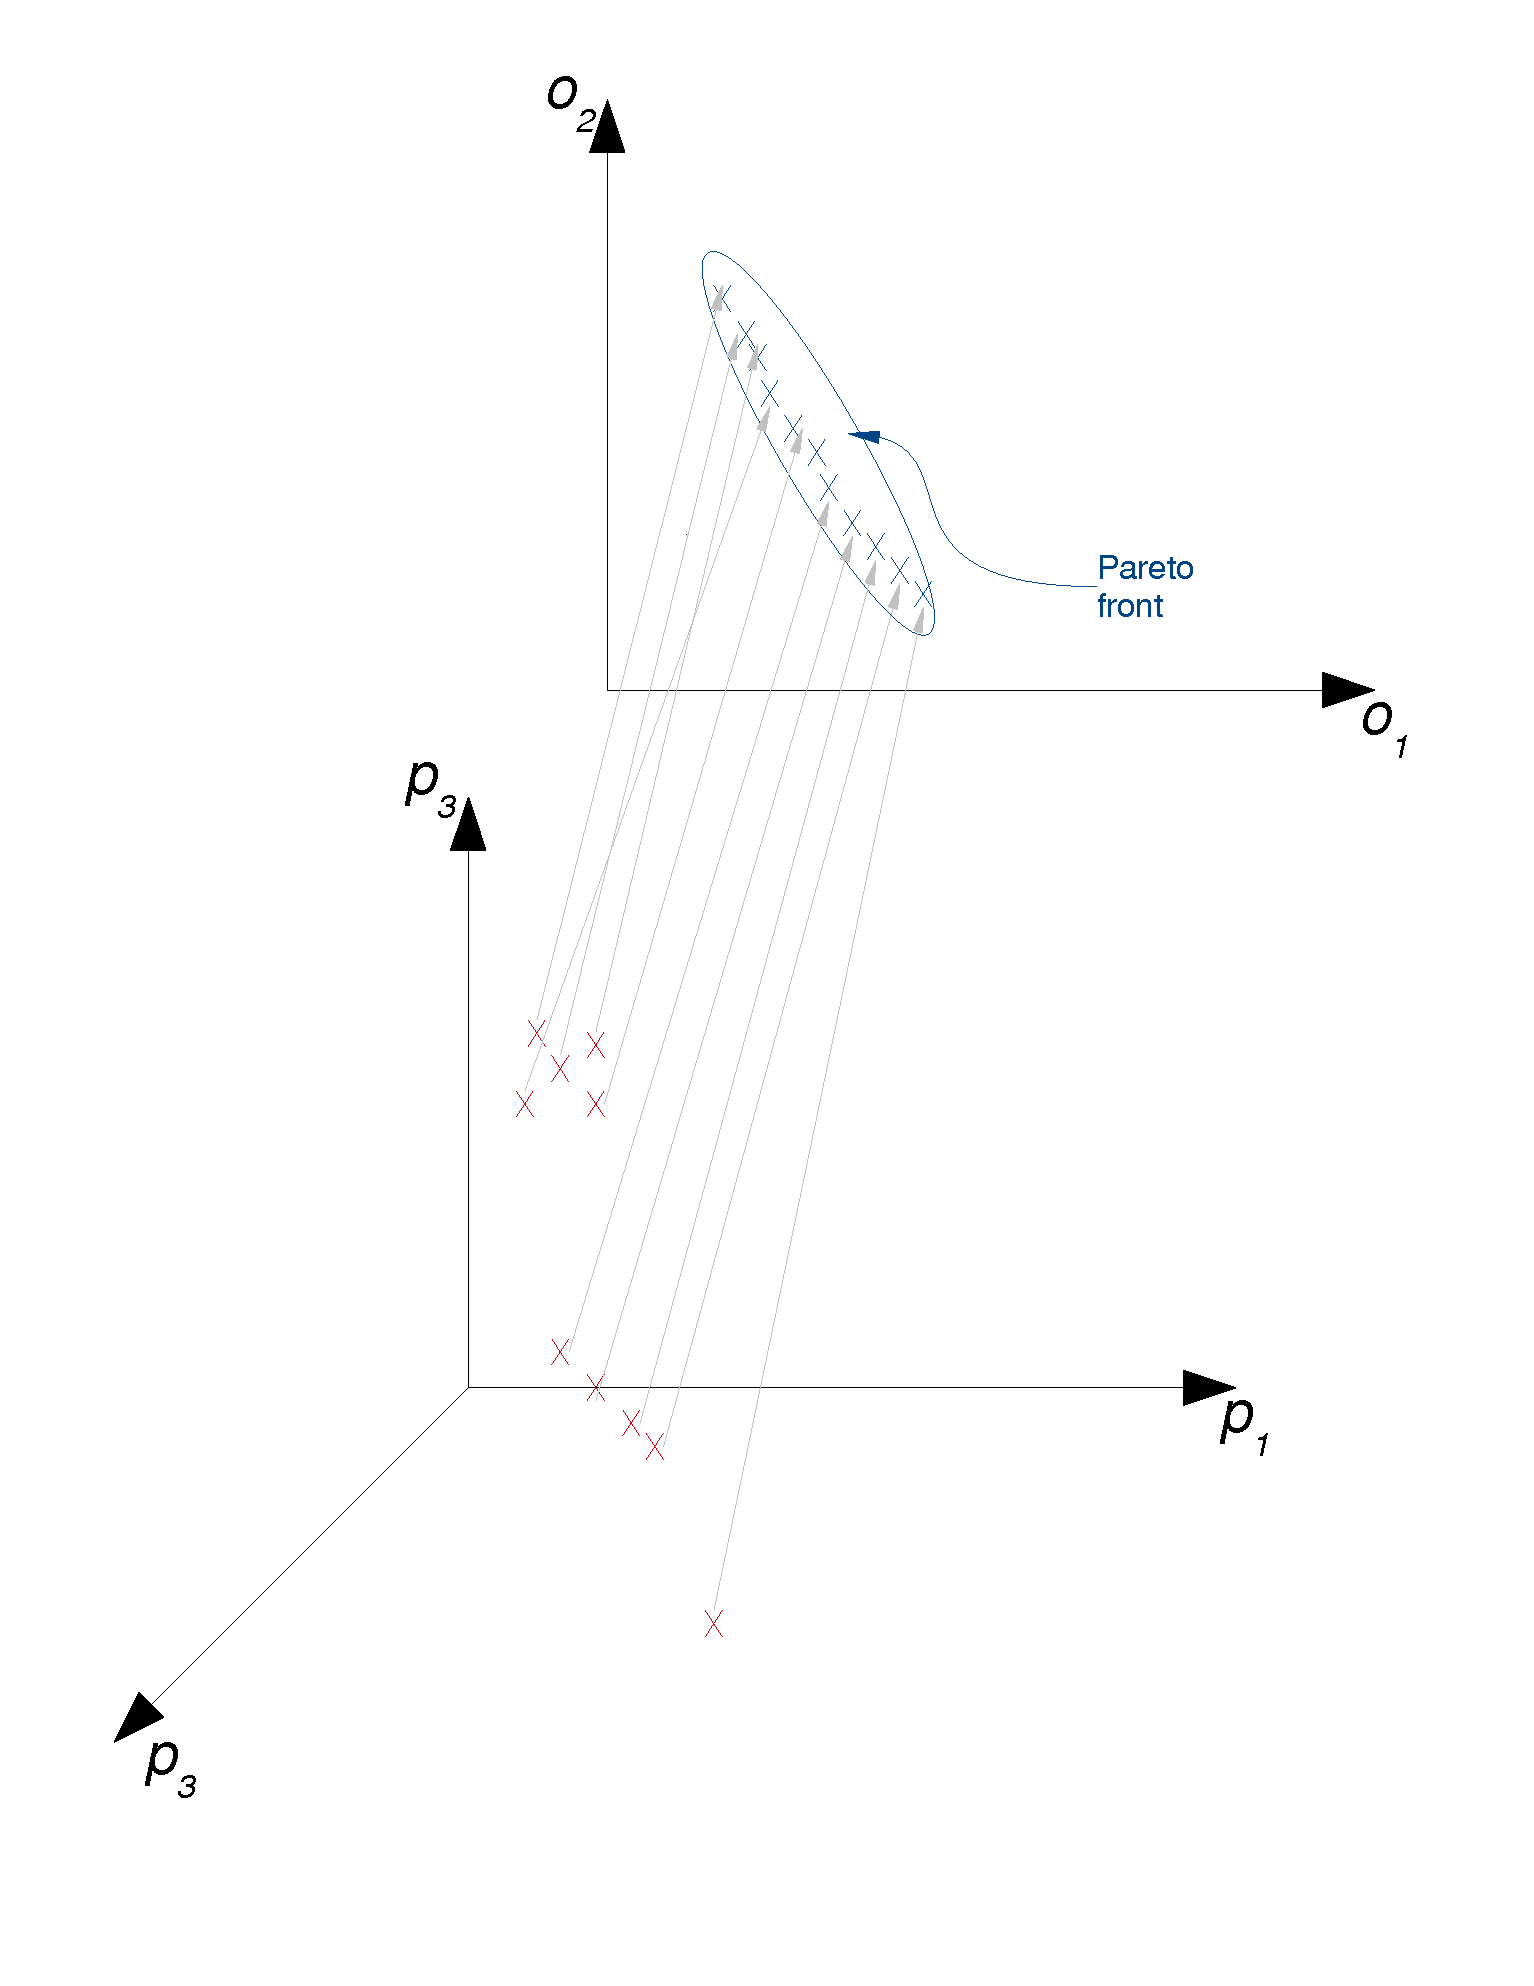
\includegraphics[width=0.9\columnwidth]{img/Pareto_set_and_front}

\caption{Relation between Pareto set (its ``parameter space representation'')
and Pareto front (``objective space representation'')}


\end{figure}



\subsection{Regions}

In the design process, there are often a lot of ``local decisions''
in which the designer can take advantage of well-known results or
heuristics. For example, in a VLIW architecture consider a configuration
with very few registers. It is well-known that, in such a condition,
increasing the number of ALUs doesn't lead to tangible better performances
but leads to an increase in area occupation. An intelligent exploration
algorithm wouldn't waste time evaluating configurations with many
ALUs and few registers. If $p_{1}$ is the parameter ``number of
registers'' and $p_{2}$ is the parameter ``number of ALUs'', we
can say that the region:
\[
R=\left\{ \left.\left(v_{1},v_{2}\right)\in P_{1}\times P_{2}\right|v_{1}<s_{1},v_{2}>s_{2}\right\} 
\]
 (where $s_{1}$ and $s_{2}$ are some threshold values) is of little
interest. This example shows that some ``dependency relation'' between
parameters may exist and can be exploited to guide the exploration:
the dependencies between parameters can suggest to the designer that,
if a parameter lies in a range, there are ranges of the other there
aren't worth exploring. Intuitively, the Cartesian product of these
ranges is an ``uninteresting region''.

The problem is that, in complex scenarios, not all relations of this
kind are known in advance. Some dependency may exist but may be hidden
to the designer. Or there may be ``local dependencies'', i.e. two
parameters may be related by a dependency but only if their values
lie on some ranges (so we can't treat them as they were related by
a true dependency). Therefore, as stated in section \ref{sec:Related-work},
setting up an exploration trying to take into account as much dependencies
as possible is a very hard task that is destined to be incompletely
accomplished. We need a methodology to ``automatically'' recognize
interesting or uninteresting regions without requiring a priori knowledge
to the designer.

We also consider, in measuring how much iteresting a region is, the
``innovation'' that it adds. If, during a design space exploration,
a Pareto front is temporarily calculated, adding a new Pareto front
point near to the previous ones is not a considerable ``innovation'',
because the way it fulfils the objectives is very similar to other
already evaluated configurations. On the contrary, adding a new Pareto
front point that is very distant from previous ones is remarkable,
because it let the experimenter realize that the objectives can be
fulfilled in a completely different way from what he already found
during exploration. So a region will be evaluated ineresting as much
as how different are its added Pareto front points from the ones already
found.
\begin{rem}
We will consider only parameters $p_{i}$ with ordering, i.e. such
that, if $P_{i}$ is a domain, $\forall a,b\in P_{i}$ it is possible
to say $a<b$ or $a=b$ or $a>b$.
\end{rem}
{[}TODO: DESCRIVERE COME SI PENSA DI TRATTARE GLI SCENARI IN CUI ESISTONO
PARAMETRI SENZA ORDINAMENTO{]}
\begin{defn}
\emph{Parameter interval}

Let $p_{i}$ be a parameter and $a_{i},b_{i}\in P_{i},a_{i}<b_{i}$.
A $p_{i}$- interval is
\[
\left[a_{i}..b_{i}\right]=\left[a_{i},b_{i}\right]\cap P_{i}
\]
 (i.e. taking the interval $\left[a_{i},b_{i}\right]$ , $\left[a_{i}..b_{i}\right]$
is the set of values of $P_{i}$ lying in $\left[a_{i},b_{i}\right]$)
\end{defn}

\begin{defn}
\emph{\label{pers02.def:Contiguous-intervals}Contiguous intervals}

Let $\left[a_{i}..b_{i}\right]$ and $\left[x_{i}..y_{i}\right]$
be two $p_{i}$-intervals. They are said to be contiguous iff
\begin{itemize}
\item $\left[a_{i}..b_{i}\right]\cap\left[x_{i}..y_{i}\right]=\emptyset$
and
\item $\left[a_{i}..b_{i}\right]\cup\left[x_{i}..y_{i}\right]$ is a $p_{i}$-
interval or $\left[x_{i}..y_{i}\right]\cup\left[a_{i}..b_{i}\right]$
is a $p_{i}$- interval
\end{itemize}
\end{defn}
\begin{figure}[h]
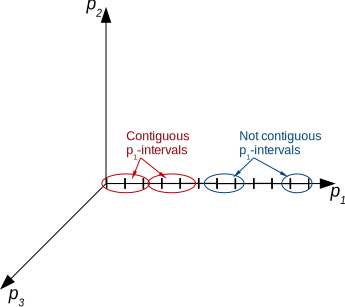
\includegraphics[width=0.9\columnwidth]{img/contiguous_intervals_or_not}

\caption{Examples of contiguous and not contiguous intervals}


\end{figure}



\begin{defn}
\emph{Region}

A region is a set of the following form:
\[
R=\left[a_{1}..b_{1}\right]\times\dots\times\left[a_{n}..b_{n}\right]=\prod\left[a_{i}..b_{i}\right]
\]
 (see figure \ref{pers02.fig:Examples-of-regions})

\begin{figure}[h]
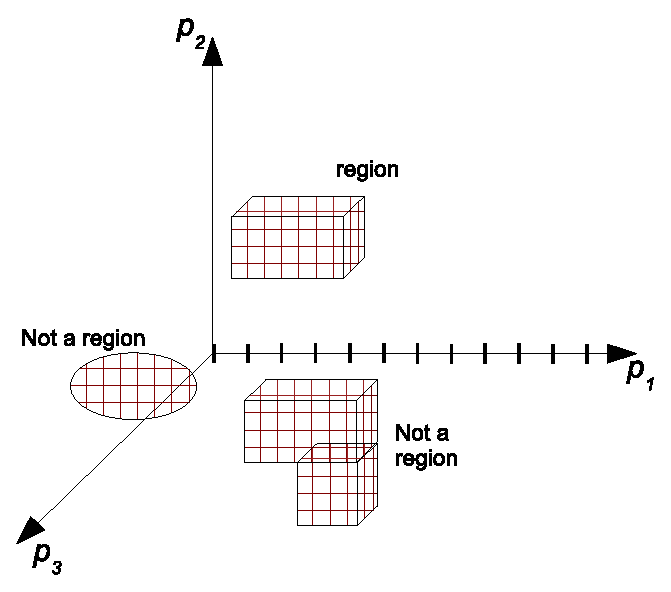
\includegraphics[width=0.9\columnwidth]{img/regions}

\caption{\label{pers02.fig:Examples-of-regions}Examples of regions}


\end{figure}
\end{defn}
\begin{rem}
We will talk later of ``big'' and ``small'' regions. The sense
of these terms is related to the cardinality of regions. A region
$R_{1}$ is said to be \emph{bigger }then $R_{2}$, if
\[
\left|R_{1}\right|>\left|R_{2}\right|
\]
 where $\left|R_{1}\right|$ and $\left|R_{2}\right|$ are the cardinalities
of $R_{1}$ and $R_{2}$. Similarly, a $p_{i}$-interval $\left[a_{i}..b_{i}\right]$
is said to be bigger then another $p_{i}$-interval $\left[c_{i}..d_{i}\right]$
if:
\[
\left|\left[a_{i}..b_{i}\right]\right|>\left|\left[c_{i}..d_{i}\right]\right|
\]


Therefore, the width of a $p_{i}$-interval $\left[a_{i}..b_{i}\right]$
is not given by the numeric value $b_{i}-a_{i}$ but it is its cardinality.
\end{rem}
We now provide some rules to split and merge regions. They will be
useful when explaining our proposed exploration algorithm.
\begin{defn}
\emph{\label{pers02.def:Splitting-a-region}Splitting a region}

If $\left[a_{i}..b_{i}\right]$ has more than one element, i.e. $\left|\left[a_{i}..b_{i}\right]\right|>1$,
it can be split in two contiguous intervals
\[
\left[a_{i}..c_{i}\right],\left[d_{i}..b_{i}\right]
\]
 such that
\[
\begin{cases}
\left[a_{i}..c_{i}\right]\cap\left[d_{i}..b_{i}\right] & =\emptyset\\
\left[a_{i}..c_{i}\right]\cup\left[d_{i}..b_{i}\right] & =\left[a_{i}..b_{i}\right]\\
\left|\left[a_{i}..c_{i}\right]\right| & =\left\lceil \frac{\left|\left[a_{i}..b_{i}\right]\right|}{2}\right\rceil 
\end{cases}
\]


If $\left|\left[a_{i}..b_{i}\right]\right|=1$ instead, the interval
cannot be split. 

If $\left[a_{i}..b_{i}\right]$ can be split, we define
\[
I_{i}=\left\{ \left[a_{i}..c_{i}\right],\left[d_{i},b_{i}\right]\right\} 
\]
 else
\[
I_{i}=\left\{ \left[a_{i}..b_{i}\right]\right\} 
\]


The whole region can be split in the following subregions
\[
\mathcal{R}^{R}=\left\{ \left.\prod\left[x_{i}..y_{i}\right]\right|\left[x_{i}..y_{i}\right]\in I_{i}\right\} 
\]


See figure \ref{pers02.fig:Splitting-a-region}.

\begin{figure}[h]
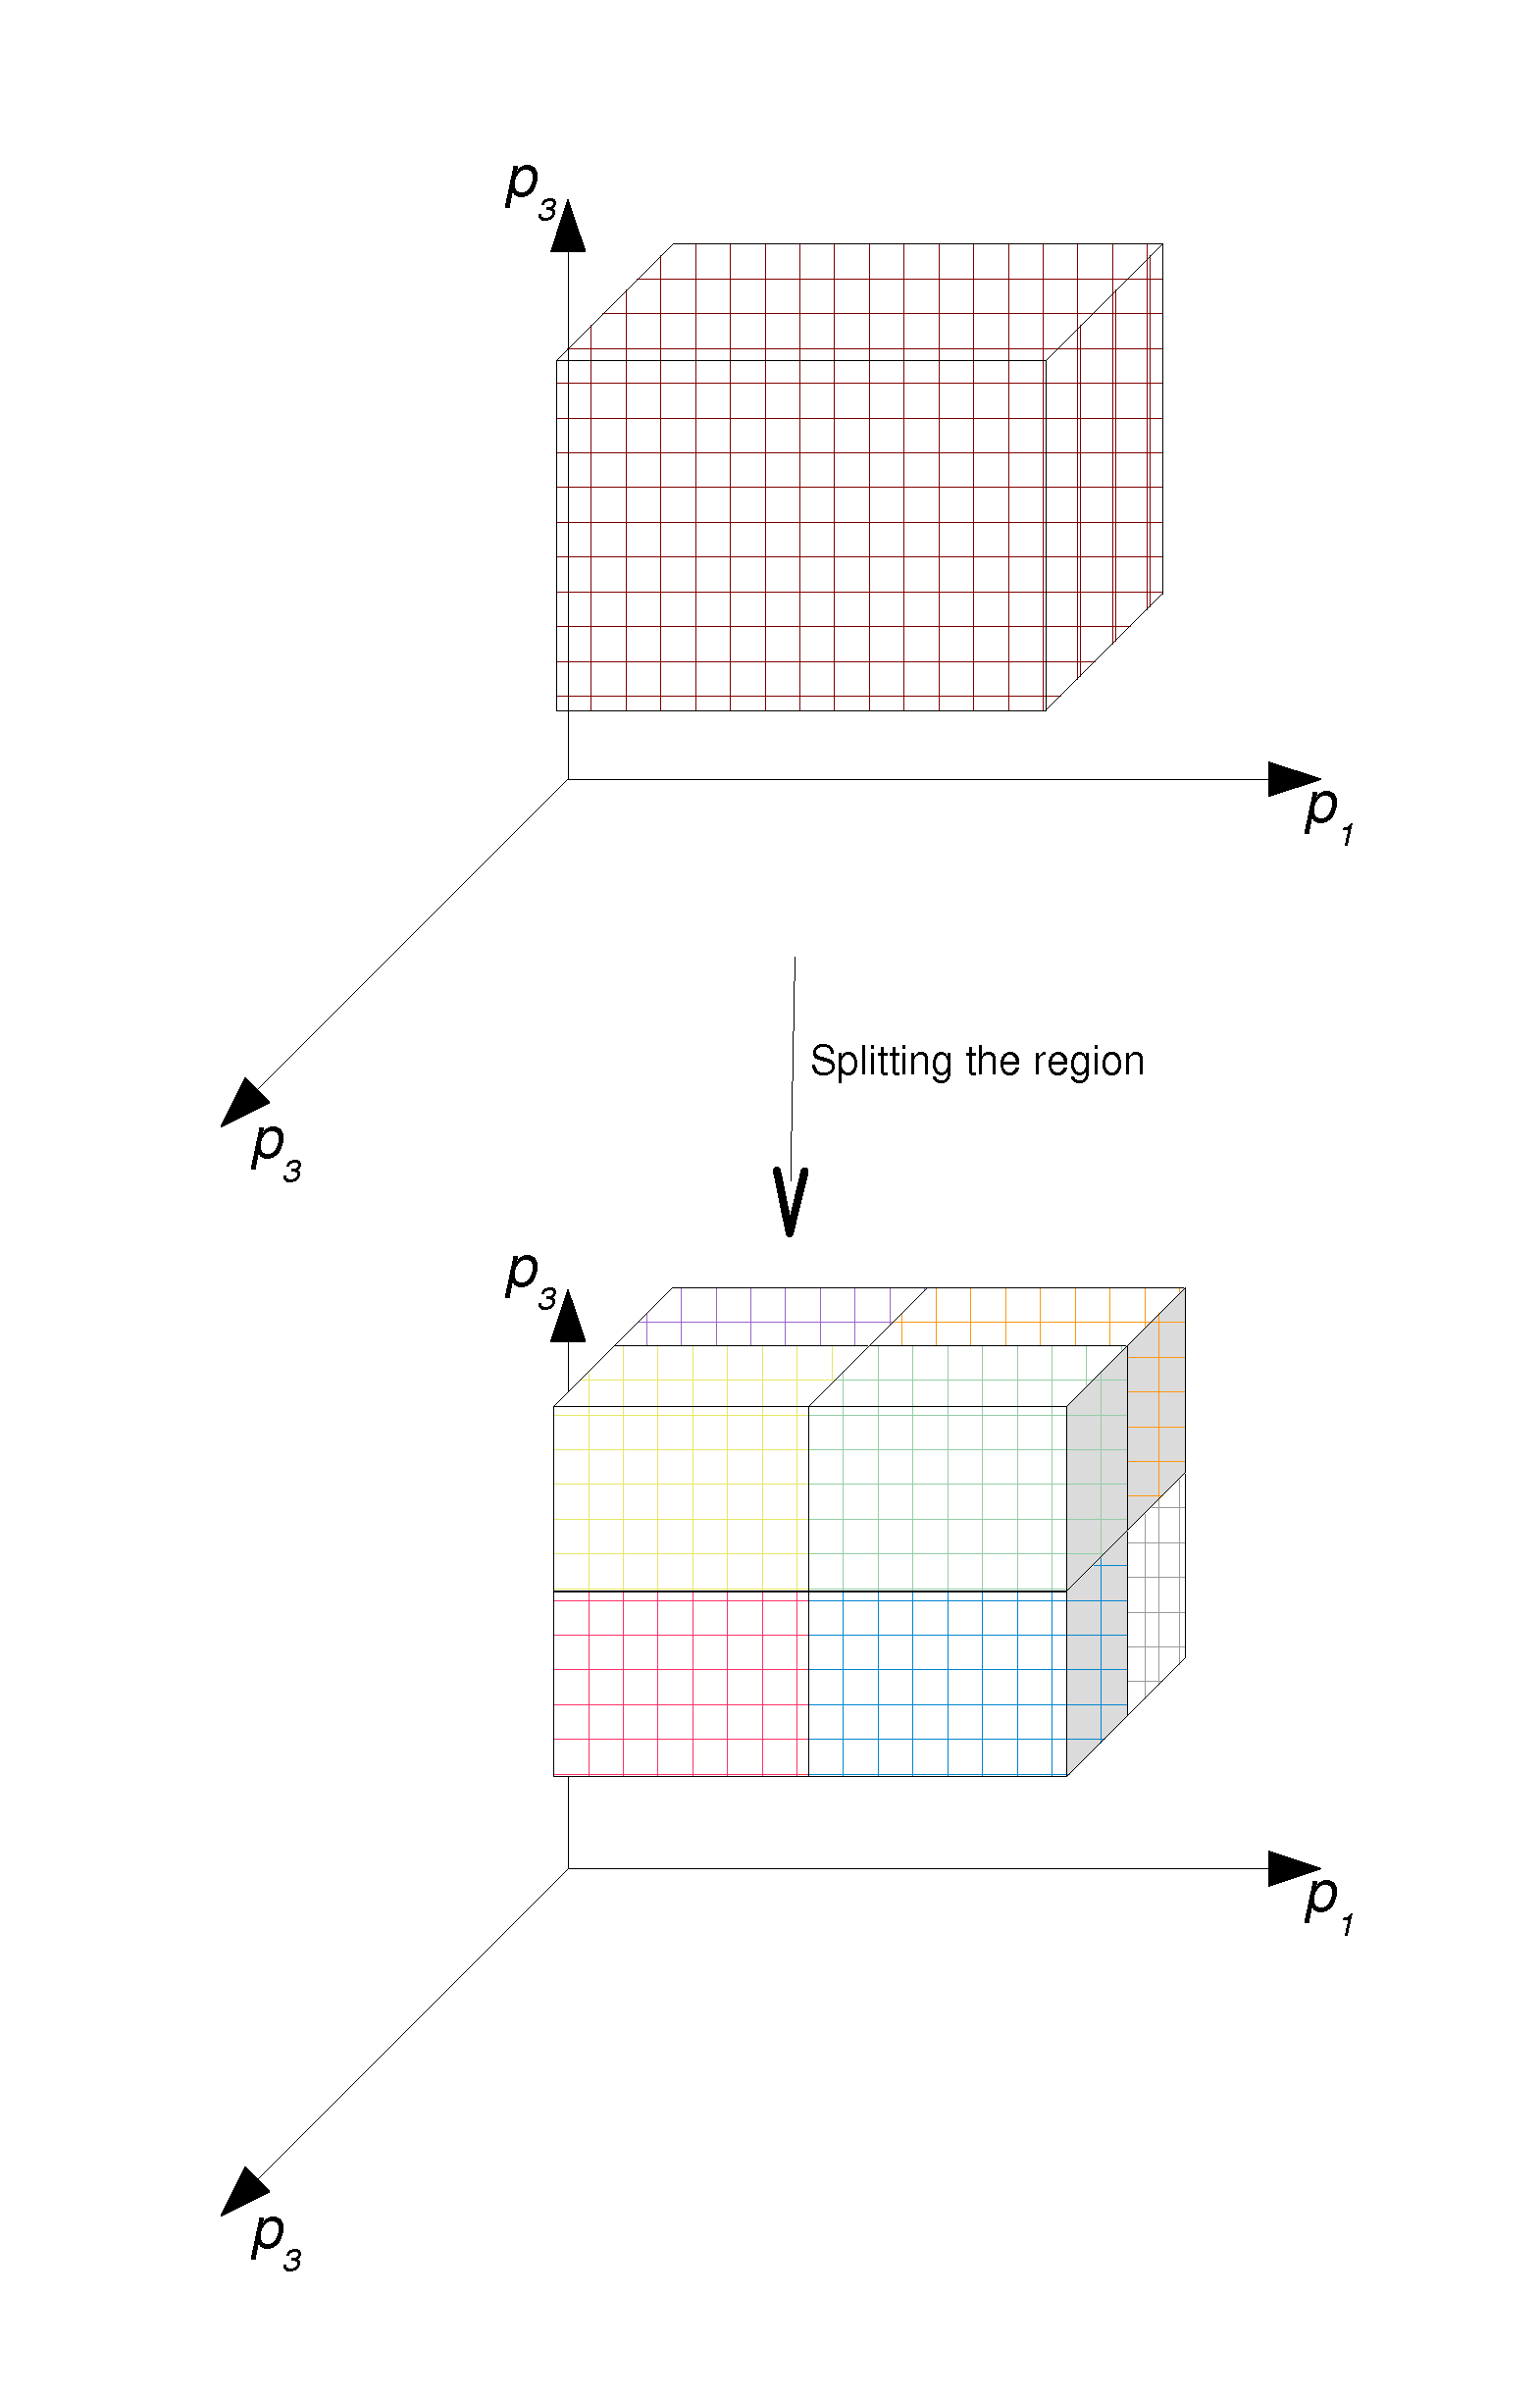
\includegraphics[width=0.9\columnwidth]{img/splitting_the_region}

\caption{\label{pers02.fig:Splitting-a-region}Splitting a region}


\end{figure}

\end{defn}

\begin{defn}
\emph{Contiguous regions}

Let $R_{1}=\prod\left[a_{i}\dots b_{i}\right]$ and $R_{2}=\prod\left[x_{i}..y_{i}\right]$
be two regions. They are said to be contiguous iff
\begin{itemize}
\item a $j$ exists such that $\left[a_{i}..b_{i}\right]=\left[x_{i}..y_{i}\right]$
for all $i\neq j$ 
\item $\left[a_{j}..b_{j}\right]$ and $\left[x_{j}..y_{j}\right]$ are
contiguous intervals (see definition \ref{pers02.def:Contiguous-intervals})
\end{itemize}
\end{defn}
See figure \ref{pers02.fig:Contiguous-regions}.

\begin{figure}[h]
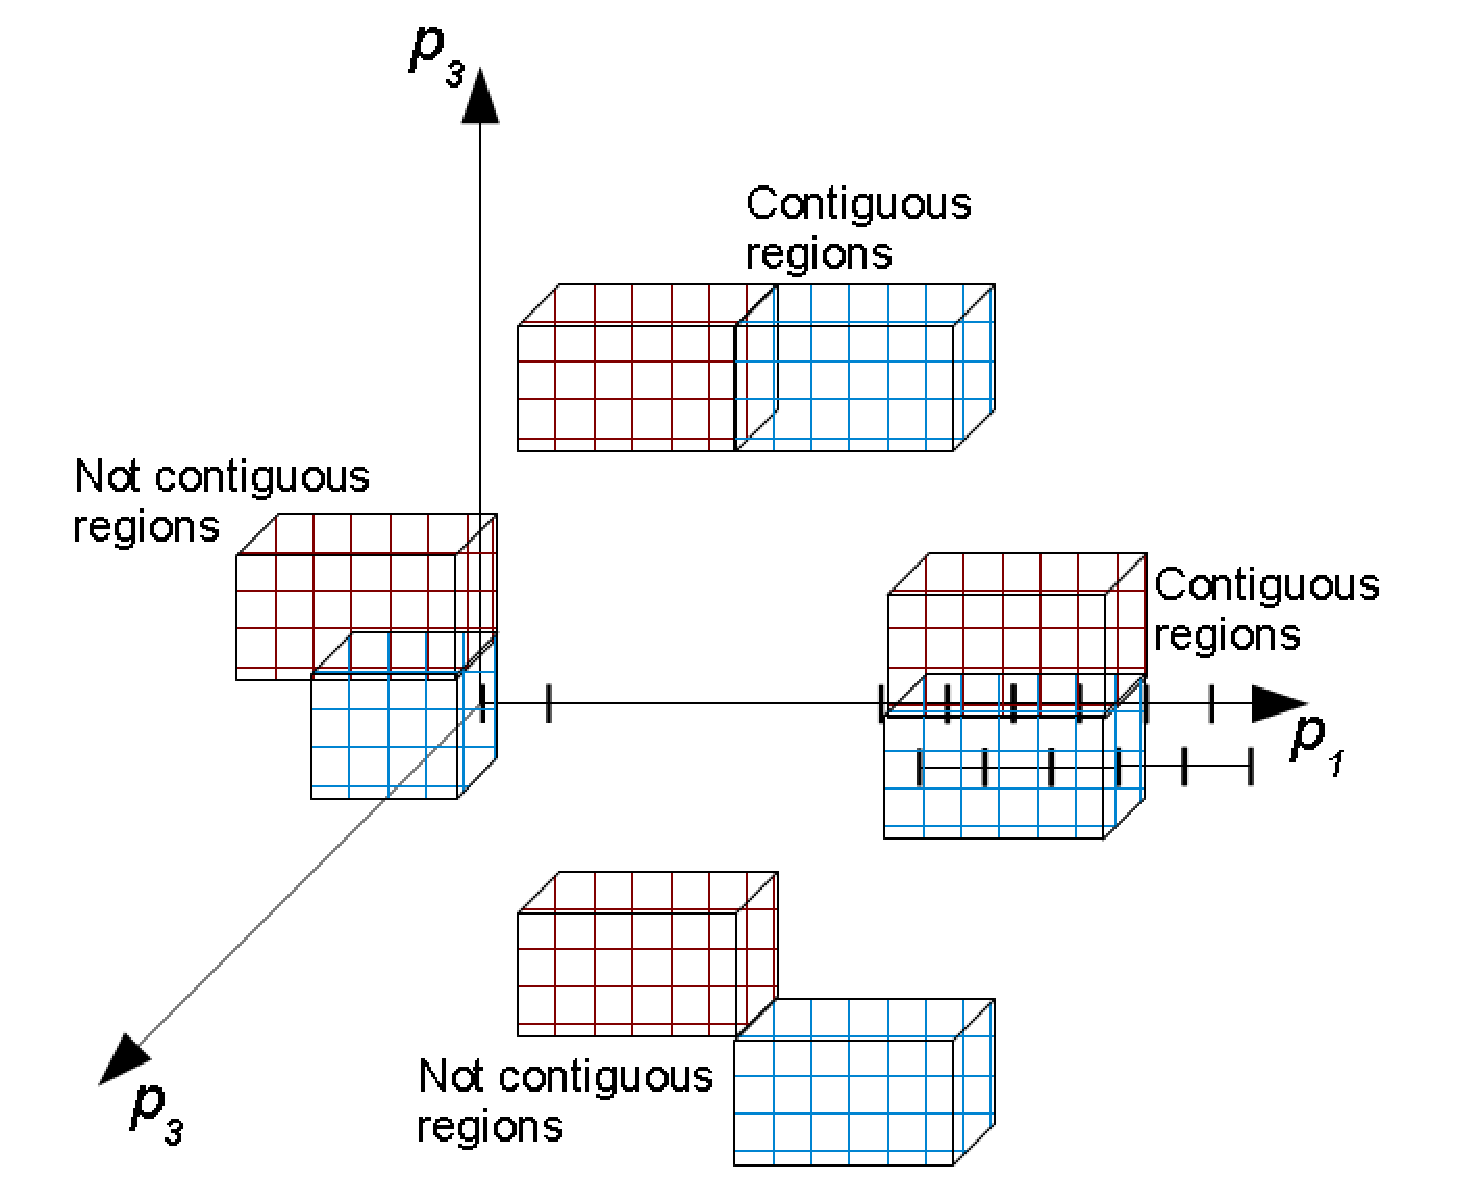
\includegraphics[width=0.9\columnwidth]{img/contiguous_regions}

\caption{\label{pers02.fig:Contiguous-regions}Contiguous and not contiguous
regions}
\end{figure}



\begin{defn}
\emph{\label{pers02.def:Merging-regions}Merging regions}

Let $R_{1}$ and $R_{2}$ be two contiguous regions as the previous
ones. Because of the definition of contiguous intervals, it is possible
that $b_{j}<x_{j}$ or $y_{j}<a_{j}$. We can merge the contiguous
intervals and obtain a new interval, as the following
\[
\left[t_{j},z_{j}\right]=\begin{cases}
\left[a_{j}..y_{j}\right] & \mbox{ if }b_{j}<x_{j}\\
\left[x_{j}..b_{j}\right] & \mbox{ if }y_{j}<a_{j}
\end{cases}
\]


The region ``$R_{1}$ merged with $R_{2}$'' is defined as
\[
R=\prod_{i<j}\left[a_{i}..b_{i}\right]\times\left[t_{j}..z_{j}\right]\times\prod_{i>j}\left[a_{i}..b_{i}\right]
\]


Such an $R$ will be indicated with the following notation:
\[
R=R_{1}+R_{2}
\]
\end{defn}
\begin{rem}
$R_{1}+R_{2}$ is mathematically equivalent to $R_{1}\cup R_{2}$.
However, using $R_{1}+R_{2}$ notation, we enforce the argument that
$R_{1}$ and $R_{2}$ must be to contiuguous regions.
\end{rem}

\begin{defn}
\emph{Separation}

Let $\mathbf{o}=\left(o_{1},\dots,o_{m}\right)$ and $\mathbf{q}=\left(q_{1},\dots,q_{m}\right)$
be two points of $O_{1}\times\dots\times O_{m}$. The separation between
$\mathbf{o}$ and $\mathbf{q}$ is 
\[
s\left(\mathbf{o}\rightarrow\mathbf{q}\right)=\sum_{i=1}^{m}\left|\frac{o_{i}-q_{i}}{o_{i}}\right|
\]


Notice that the separation is not a commutative operator.\end{defn}
\begin{rem}
The separation between $\mathbf{o}$ and $\mathbf{q}$ measures how
much we must vary $\mathbf{o}$ to transfrom it in $\mathbf{q}$.
The separation is a ``normalized'' measure that is independent of
the nature and the unit of measurement of the objectives
\end{rem}

\begin{defn}
\emph{Separation (alternative)}

Another definition of separation could be:
\[
s\left(\mathbf{o}\rightarrow\mathbf{q}\right)=\max_{i=1,\dots,m}\left|\frac{o_{i}-q_{i}}{o_{i}}\right|
\]

\end{defn}

\section{The algorithm}

The algorithm we present is iterative. Each iteration is called \emph{era}. 

Each era $era_{i}$ is characterized by 
\begin{itemize}
\item the set of regions $\mathcal{R}_{i}$ in which the parameter space
$P_{1}\times\dots\times P_{n}$ is divided
\item its Pareto set $\mathscr{P}_{i}$
\item a set $test_{i}$ of at most $K$ configurations to evaluate
\end{itemize}
$K$ is a parameter that must be set before the algorithm runs.


\paragraph{START CONDITION}
\begin{itemize}
\item $\mathcal{R}_{0}=\left\{ P_{1}\times\dots\times P_{n}\right\} $,
i.e. era $0$ has only one region that is the whole parameter space.
A random set $test_{0}$ of $K$ configurations is evaluated. The
Pareto set $\mathscr{P}_{0}=\mathscr{P}\left(test_{0}\right)$ is
calculated (see def \ref{pers02.def:Pareto-set} for the definition
of the operator $\mathscr{P}_{i}$ over a set)
\end{itemize}

\paragraph{ITERATION RULES}

For $era_{i}$ with $i>0$ the following operations must be performed.
\begin{enumerate}
\item \label{pers02.enu:K}For each region $R\in\mathcal{R}_{i}$, a set
$test_{R,i}$ of configurations is randomly chosen in%
\footnote{Therefore the chosen configurations can only be configurations of
$R$ not yet evaluated in past eras.%
} $R\setminus\bigcup_{j=0}^{i-1}test_{j}$. The number of configurations
in $test_{R,i}$ is set to%
\footnote{This means that $\frac{K}{\left|\mathcal{R}_{i}\right|}$ configurations
are to be chosen, but if not yet evaluated configurations in $R$
are less then $\frac{K}{\left|\mathcal{R}_{i}\right|}$, all of them
are chosen%
} 
\[
\min\left(\frac{K}{\left|\mathcal{R}_{i}\right|},\left|R\setminus\bigcup_{j=1}^{i-1}test_{j}\right|\right)
\]
The set 
\[
test_{i}=\bigcup_{R\in\mathcal{R}_{i}}test_{R,i}
\]
 is defined. 
\item All configurations on $test_{i}$ are simulated.
\item The Pareto set $\mathscr{P}_{i}$ for $era_{i}$ is defined as 
\[
\mathscr{P}_{i}=\mathscr{P}\left(test_{i}\cup\mathscr{P}_{i-1}\right)
\]

\item \label{pers02.enu:novelty_score_of_a_configuration}Every point $\mathbf{p}$
of%
\footnote{The innovation score is not given to those points in $test_{i}$ that
are not in the Pareto set%
} $test_{i}\cap\mathscr{P}_{i}$ is given an \emph{innovation score
}defined as:
\[
is\left(\mathbf{p}\right)=\min\left\{ \left.s\left(\mathbf{q}\rightarrow\mathbf{o}\left(\mathbf{p}\right)\right)\right|\mathbf{q}\in\mathscr{P}_{i-1}\right\} 
\]
 (a configuration $\mathbf{p}$ is characterized by as much innovation
as more separated it is from the configurations of the previous era)\@.
\item Every region $R\in\mathcal{R}_{i}$ is given an innovation score defined
as:
\[
is\left(R\right)=\sum\left\{ \left.is\left(\mathbf{p}\right)\right|\mathbf{p}\in\mathscr{P}_{i}\cap R\right\} 
\]

\item The total innovation score for the entire era is:
\[
is_{TOT,i}=\sum_{R\in\mathcal{R}_{i}}is\left(R\right)
\]

\item The avarage innovation score for the entire era is also calculated
as:
\[
is_{av,i}=\frac{is_{TOT,i}}{\left|\mathcal{R}_{i}\right|}
\]
where $\left|\mathcal{R}_{i}\right|$ is the number of regions of
era $i$ .
\item $\mathcal{R}_{i}$ is partitioned in three subsets (their meaning
will be discussed later):

\begin{enumerate}
\item high innovation regions 
\[
\mathcal{R}_{i,h}=\left\{ \left.R\in\mathcal{R}_{i}\right|is\left(R\right)>\alpha\cdot is_{av,i-1}\right\} 
\]
 where $\alpha$ is a constant defined by the designer (for example
$\alpha=1.2$). Each $R\in\mathcal{R}_{i,h}$ is split in $\mathcal{R}^{R}$
(as stated in def \ref{pers02.def:Splitting-a-region})
\item low innovation regions 
\[
\mathcal{R}_{i,l}=\left\{ \left.R\in\mathcal{R}_{i}\right|0<is\left(R\right)\le\alpha\cdot is_{av,i-1}\right\} 
\]
They are not changed.
\item no innovation regions 
\[
\mathcal{R}_{i,n}=\left\{ \left.R\in\mathcal{R}_{i}\right|is\left(R\right)=0\right\} 
\]

\end{enumerate}
\item Disjoint couples of contiguous regions $\left(R_{1},R_{2}\right)$,
with $R_{1},R_{2}\in\mathcal{R}_{i,n}$ are selected. The set of this
couples is indicated as $\mathcal{C}$. The couples of regions are
merged:
\[
\forall\left(R_{1},R_{2}\right)\in\mathcal{C}\Rightarrow R=R_{1}+R_{2}
\]
 (see def \ref{pers02.def:Merging-regions})
\item The set of regions $\mathcal{R}_{i+1}$ for the following era is defined
as:
\[
\mathcal{R}_{i+1}=
\]
\[
=\left(\bigcup_{R\in\mathcal{R}_{i,h}}\mathcal{R}^{R}\right)\cup\mathcal{R}_{i,l}\cup
\]
\[
\cup\left(\mathcal{R}_{i,n}\setminus\bigcup_{\left(R_{1},R_{2}\right)\in\mathcal{C}}\left\{ R_{1},R_{2}\right\} \right)\cup
\]
\[
\cup\left(\bigcup_{\left(R_{1},R_{2}\right)\in\mathcal{C}}\left(R_{1}+R_{2}\right)\right)
\]

\end{enumerate}

\paragraph{TERMINATION CONDITION}
\begin{itemize}
\item The algorithm terminates at step $k$ if
\[
is_{TOT,k},is_{TOT,k-1},\dots,is_{TOT,k-\beta}\le\gamma\cdot is_{TOT,k-\left(\beta-1\right)}
\]
 where $\beta$ and $\gamma$ are selected by the experimenter (see
remark \ref{rem:termination}).\end{itemize}
\begin{rem}
\label{pers02.rem:smaller_regions}The rule \ref{pers02.enu:K} of
the iteration rules says that the smaller is a region, the more ``crowded''
it is. It means that configurations in smaller regions are evaluated
with more ``attention'' (see figure \ref{pers02.fig:small_and_big}).

\begin{figure}[h]
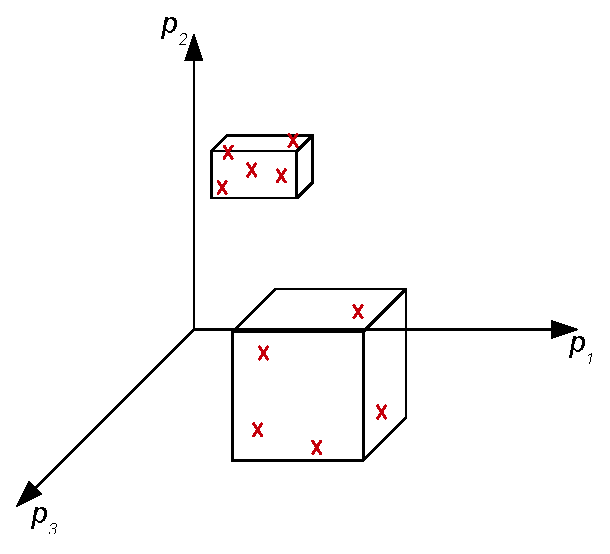
\includegraphics[width=0.9\columnwidth]{img/small_and_big}

\caption{\label{pers02.fig:small_and_big}In this example 5 configurations
are evaluated in a small region and in a bigger region. In can be
seen that smaller region is more crowded.}


\end{figure}

\end{rem}

\begin{rem}
The rule \ref{pers02.enu:novelty_score_of_a_configuration} says that
a configuration whose objectives are more ``separated'' by the previous
Pareto front, has to be taken in greater account than others. A configuration
that is very near, in the objective space, to the previous Pareto
front doesn't add a true innovation. Therefore, the innovation score
of a configuration is a measure of how much interest we have in considering
it (see figure \ref{pers02.fig:Novelty-score-of-a-config}).

\begin{figure}[h]
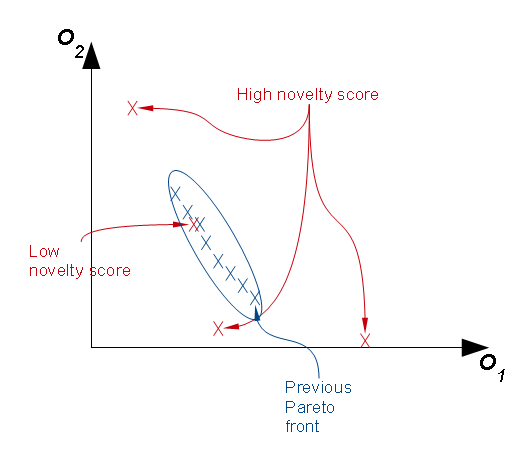
\includegraphics[width=0.9\columnwidth]{img/novelty_score}

\caption{\label{pers02.fig:Novelty-score-of-a-config}innovation score of a
configuration}


\end{figure}

\end{rem}

\begin{rem}
The innovation score of a region is a measure of how much different
are the points that it adds to Pareto Front compared to the previous
Pareto front. ``High innovation regions'' are the ones in which
more configurations are worth evaluating, because they add many points
on not yet well explored Pareto front areas. Therefore, these regions
are split in the next era (see remark \ref{pers02.rem:smaller_regions})
and more ``crowded'' by simulations. ``No innovation regions''
are the ones that have proved to add few points on Pareto fronts,
probably very near to previous Pareto front points and a Pareto front
point near to previous points is not so much interesting. Therefore
it's not worth evaluating many of their configurations and it is useful
to merge these regions , in order to less densely evaluate them.

ULTERIORI GIUSTIFICAZIONI SULL'IMPORTANZA DI CONSIDERARE LA DIVERSITA'
DELLE SOLUZIONI SI TROVA IN ext12.pag5 E ALTRI.
\end{rem}

\begin{rem}
\label{rem:termination}The algorithm terminates when in the last
$\beta$ iterations not a great ``amount of innovation'' has been
discovered. Therefore it is very probably that carrying on iterating
will not considerably change the Pareto front already formed. It's
not recommended to chose $\beta=1$, because it is possible that the
Pareto fronts $\mathbf{o}\left(\mathscr{P}_{k-1}\right)$ and $\mathbf{o}\left(\mathscr{P}_{k}\right)$
are not very different but next Pareto fronts could be. In other words,
it's unsafe to terminate as soon as the Pareto front doesn't change
enough, passing from an era to the next. It's better taking into account
more than one era.
\end{rem}
!!! IN INGLESE E' PIU' CORRETTO DIRE: ``IT IS POSSIBLE THAT THE PARETO
FRONTS WERE NOT VERY DIFFERENT''? (CON ``WERE'' AL POSTO DI ``ARE'')


\begin{rem}
Merging and splitting the regions are very dynamic processes. A portion
of the parameter space can be populated by a large number of small
regions in some eras, but can be covered by a small number of large
regions in next eras. This can be explained saying that, after a number
of eras of intense exploration of a portion of parameter space, this
exploration has turned to be enough thorough and so it was time for
other portions to be minutely scanned.
\end{rem}

\section{Experiments}


\section{Conclusions}
This is the end

\balance

\bibliographystyle{IEEEtran} 
\bibliography{bibliography}

% TODO: G2012 bib not used ?

\end{document}
